Sei $ABC$ ein Dreieck mit $AB=AC$ und sei $M$ der Mittelpunkt der Strecke $BC$. Sei $P$ ein Punkt, sodass $PB<PC$ gilt und $PA$ parallel zu $BC$ ist. Ferner seien $X$ und $Y$ Punkte auf den Geraden $PB$ respektive $PC$, sodass $B$ auf der Strecke $PX$ und $C$ auf der Strecke $PY$ liegt und $\angle PXM = \angle PYM$ gilt. Zeige, dass $APXY$ ein Sehnenviereck ist.

\textbf{Erste Lösung:} (Patrick by David):
Wir führen den Punkt $Z$ ein, der der zweite Schnittpunkt der Kreise durch $MCY$ und $MXB$ ist. Mit Winkeljagd folgt nun, $\angle MZC = \angle MYC = \angle MXB = \angle MZB$. Somit liegt M auf der Mittelsenkrechten von $BC$. Folglich gilt 
\[ \angle ZXP = \angle ZXB = \angle ZMB = \angle ZMC = \angle ZYC = = \angle ZYP = 90 ^\circ = \angle ZAP.
\]
Die Punkte $A$,$X$,$Y$ liegen somit auf einem Kreis mit Durchmesser $PZ$. Somit ist $PAXY$ ein Sehnenviereck.

\begin{center}
 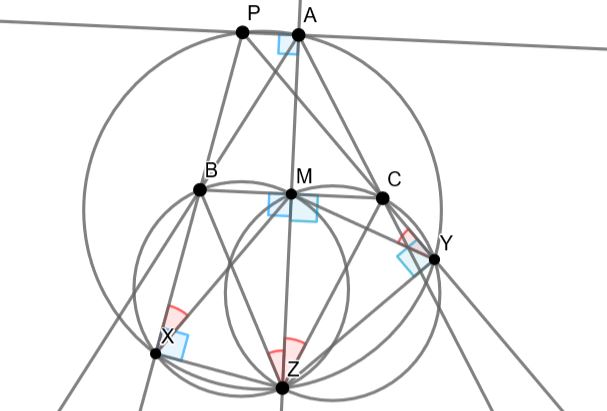
\includegraphics[width=10cm]{solutions/s5_picture.JPG}
\end{center}

\textbf{Marking scheme (Erste Lösung):}
\begin{itemize}
\item 3P: Einführung des Punktes $Z$ als Schnittpunkt der beiden Kreise
\item 1P: Feststellung, dass $ZBC $ein gleichschenkliges Dreieck ist.
\item 1P: Feststellung, dass $Z$ auf $AM$ liegt.
\item 2P: Schlussfolgern, dass $ZXYPA$ auf einem Kreis liegen.
\begin{itemize}
    \item 1P: Folgern, dass $P, Z$ mit zwei der anderen drei Punkten auf einem Kreis liegen
\end{itemize}
%% einen Punkt wenn nur XYPZ auf einem Kreis liegen ? 
\end{itemize}